\chapter{Descrierea problemei și abordări existente}\label{chapter:cap3} %{Materiale și metodă}

Acest capitol detaliază particularitățile problemei de clasificare abordate în lucrare, punând accent pe similaritățile morfologice pronunțate dintre cele două specii vizate și pe dificultățile pe care acestea le generează în procesul de identificare. Este realizată, în continuare, o analiză critică a unor lucrări recente din literatură care abordează probleme conexe de identificare automată a racilor prin tehnici de deep learning, bazate pe arhitecturi din familia YOLO. Pentru fiecare lucrare discutată sunt prezentate metodologia, rezultatele obținute și principalele limitări, urmate de o comparație explicită cu modul în care abordarea propusă în această lucrare se diferențiază prin natura problemei, speciile vizate și condițiile de colectare a datelor.

\section{Particularități ale problemei}

Identificarea speciilor de rac din imagini depinde de evidențierea caracteristicilor morfologice relevante, precum forma rostrului, structura cleștilor și conturul cefalotoracelui \cite{parvulescu2009}. Vizibilitatea acestor elemente este influențată de unghi, lumină și calitatea imaginii.

Cele două specii vizate, \textit{Austropotamobius bihariensis} și \textit{Austropotamobius torrentium}, prezintă similarități morfologice pronunțate: ambele au crusta netedă, creasta postorbitală discretă fără spin și rostrul de formă triunghiulară \cite{parvulescu2009}. Diferențele constau în detalii fine, precum lungimea relativă a solzului antenal față de articolele bazale ale antenei și gradul de rugozitate al chelelor, caractere care nu sunt vizibile în toate imaginile, în special atunci când exemplarul este parțial acoperit sau capturat dintr-un unghi nefavorabil.

Asemănările morfologice dintre specii impun analiza unor detalii fine, care nu sunt vizibile în toate imaginile. Identificarea corectă presupune localizarea regiunilor relevante și extragerea trăsăturilor utile pentru clasificare. O dificultate suplimentară este reprezentată de variabilitatea intraspecifică de colorit: \textit{A. torrentium} poate varia de la brun-închis la portocaliu-deschis sau chiar albicios \cite{parvulescu2009}, ceea ce reduce fiabilitatea culorii ca trăsătură discriminatorie și crește importanța caracteristicilor de formă și textură.


Figura~\ref{fig:specii_raci} ilustrează exemplare reprezentative din cele două specii, evidențiind atât similaritatea morfologică generală, cât și variabilitatea de colorit discutată anterior.

\begin{figure}[H]
    \centering
    \begin{subfigure}{0.45\textwidth}
        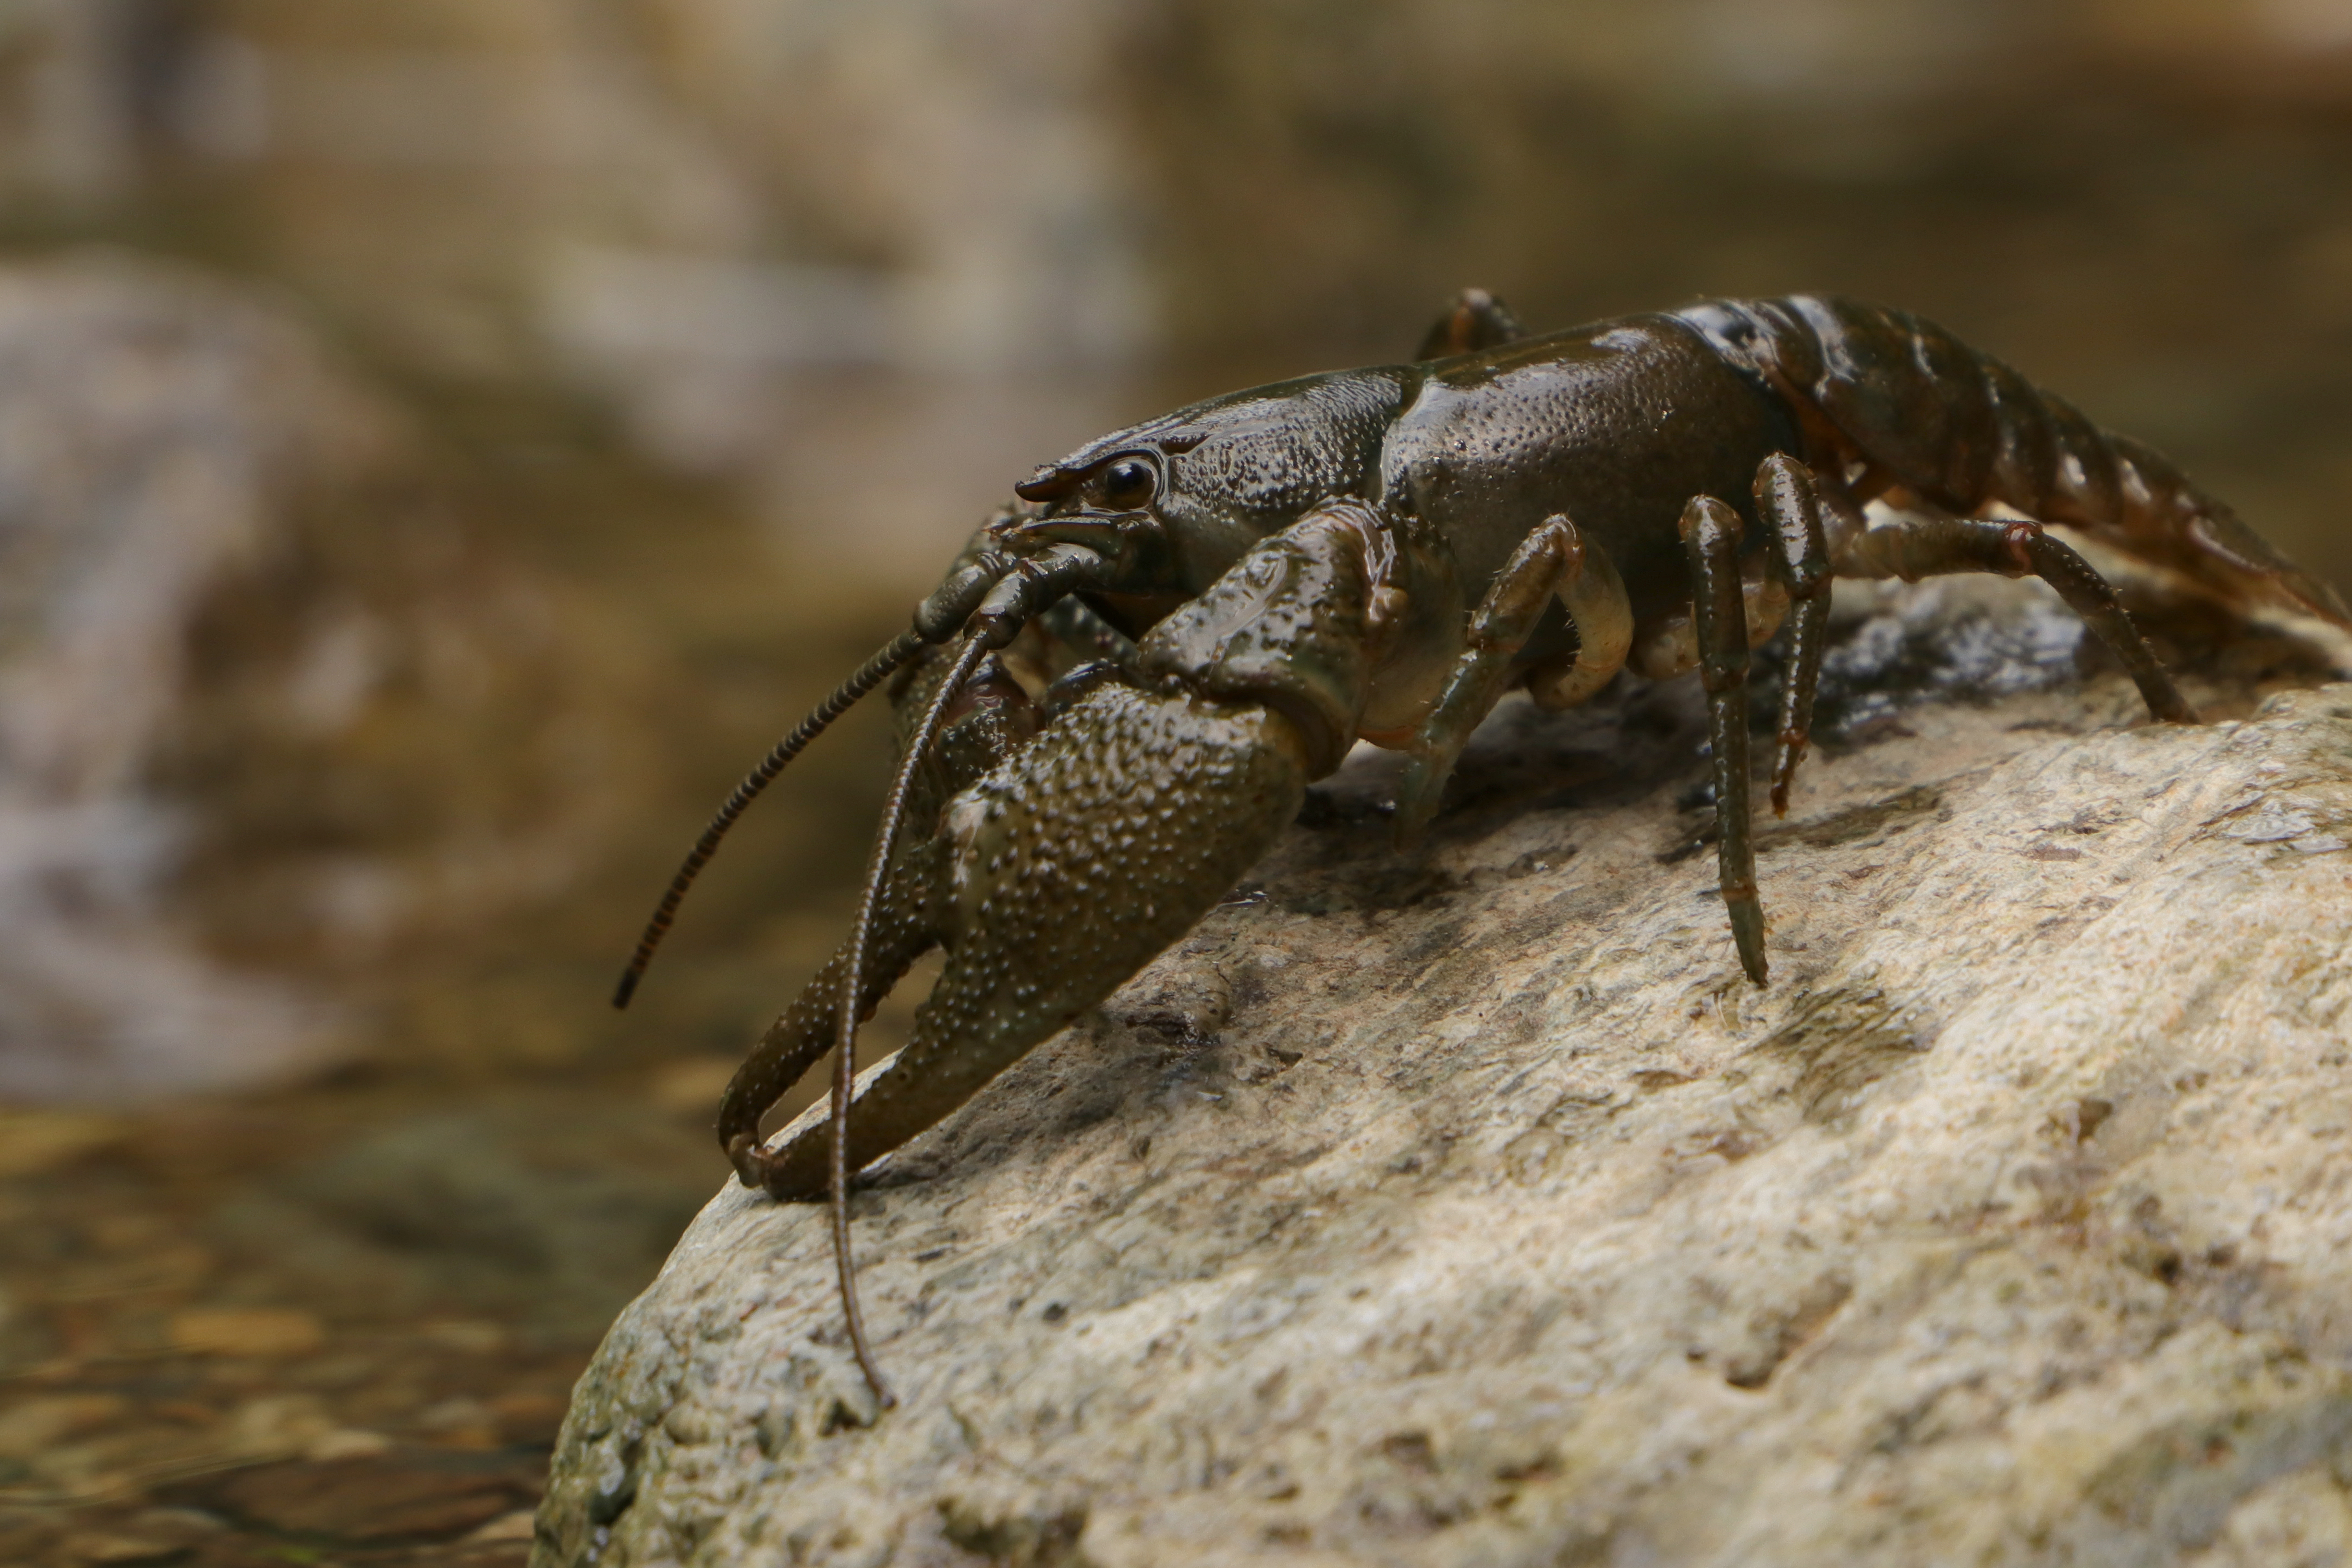
\includegraphics[width=\textwidth]{figs/Bihariensis_ex1.jpg}
    \end{subfigure}
    \hfill
    \begin{subfigure}{0.45\textwidth}
        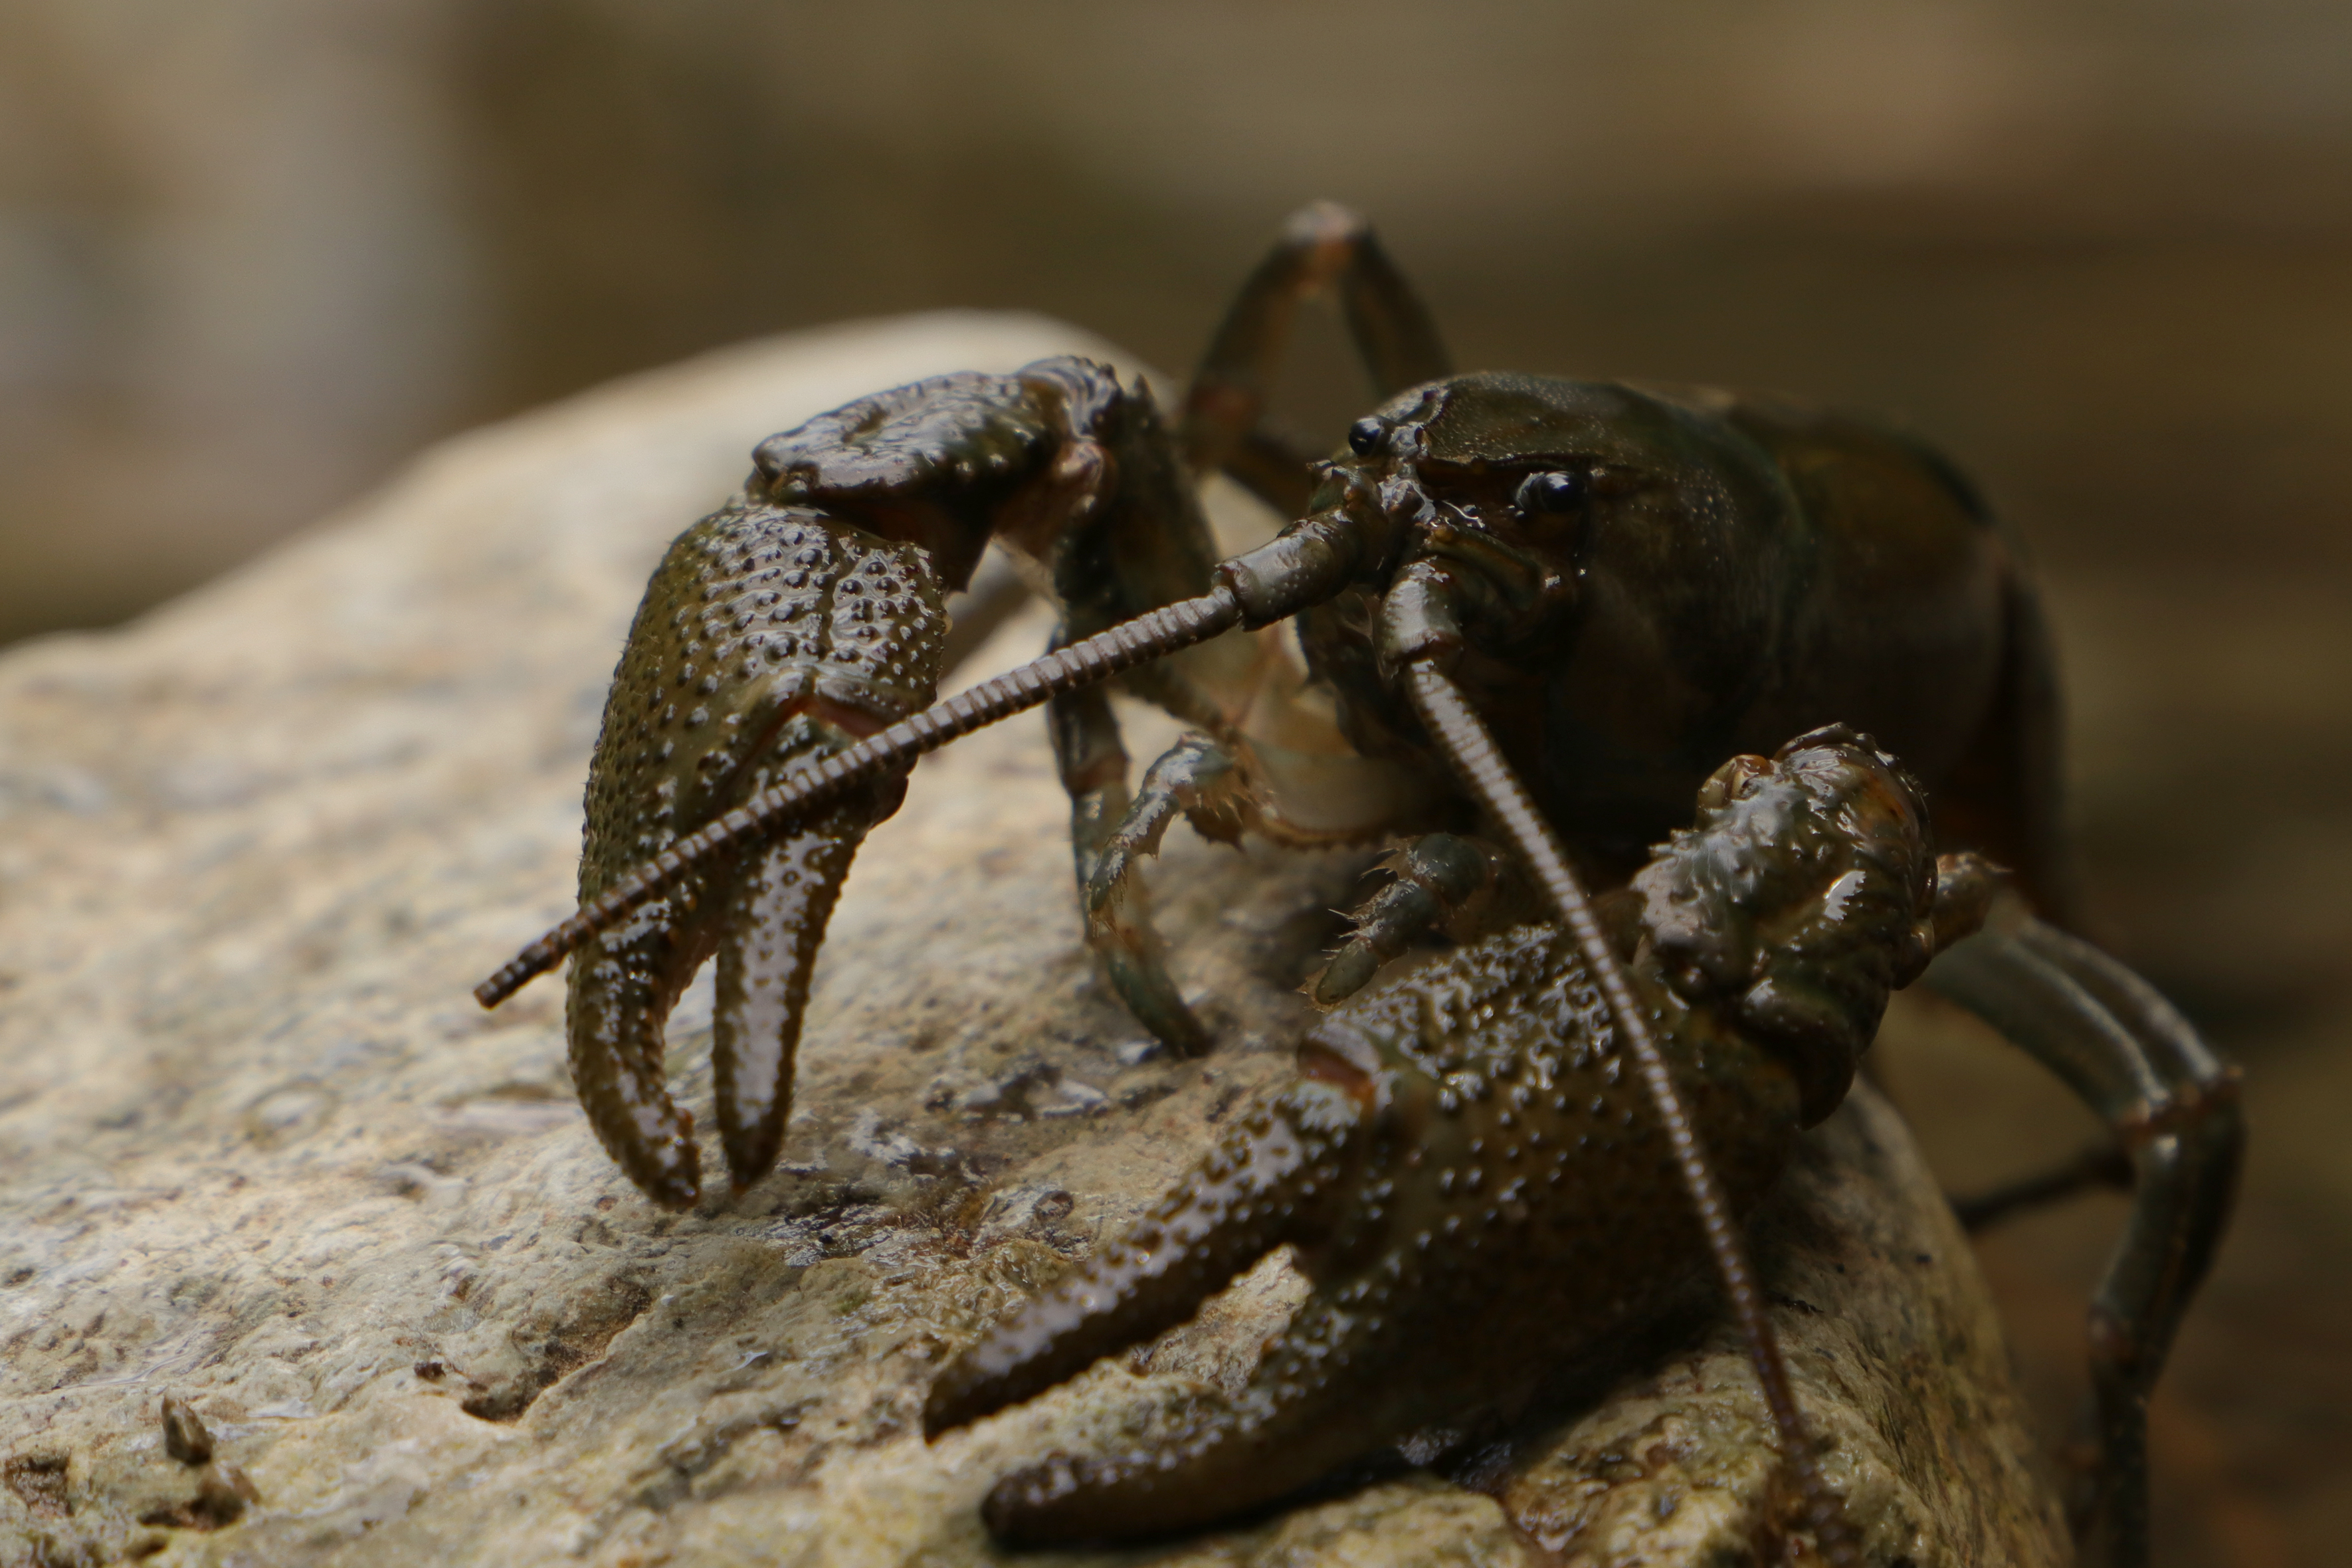
\includegraphics[width=\textwidth]{figs/Bihariensis_ex2.jpg}
    \end{subfigure}

    \vspace{0.5em}

    \begin{subfigure}{0.45\textwidth}
        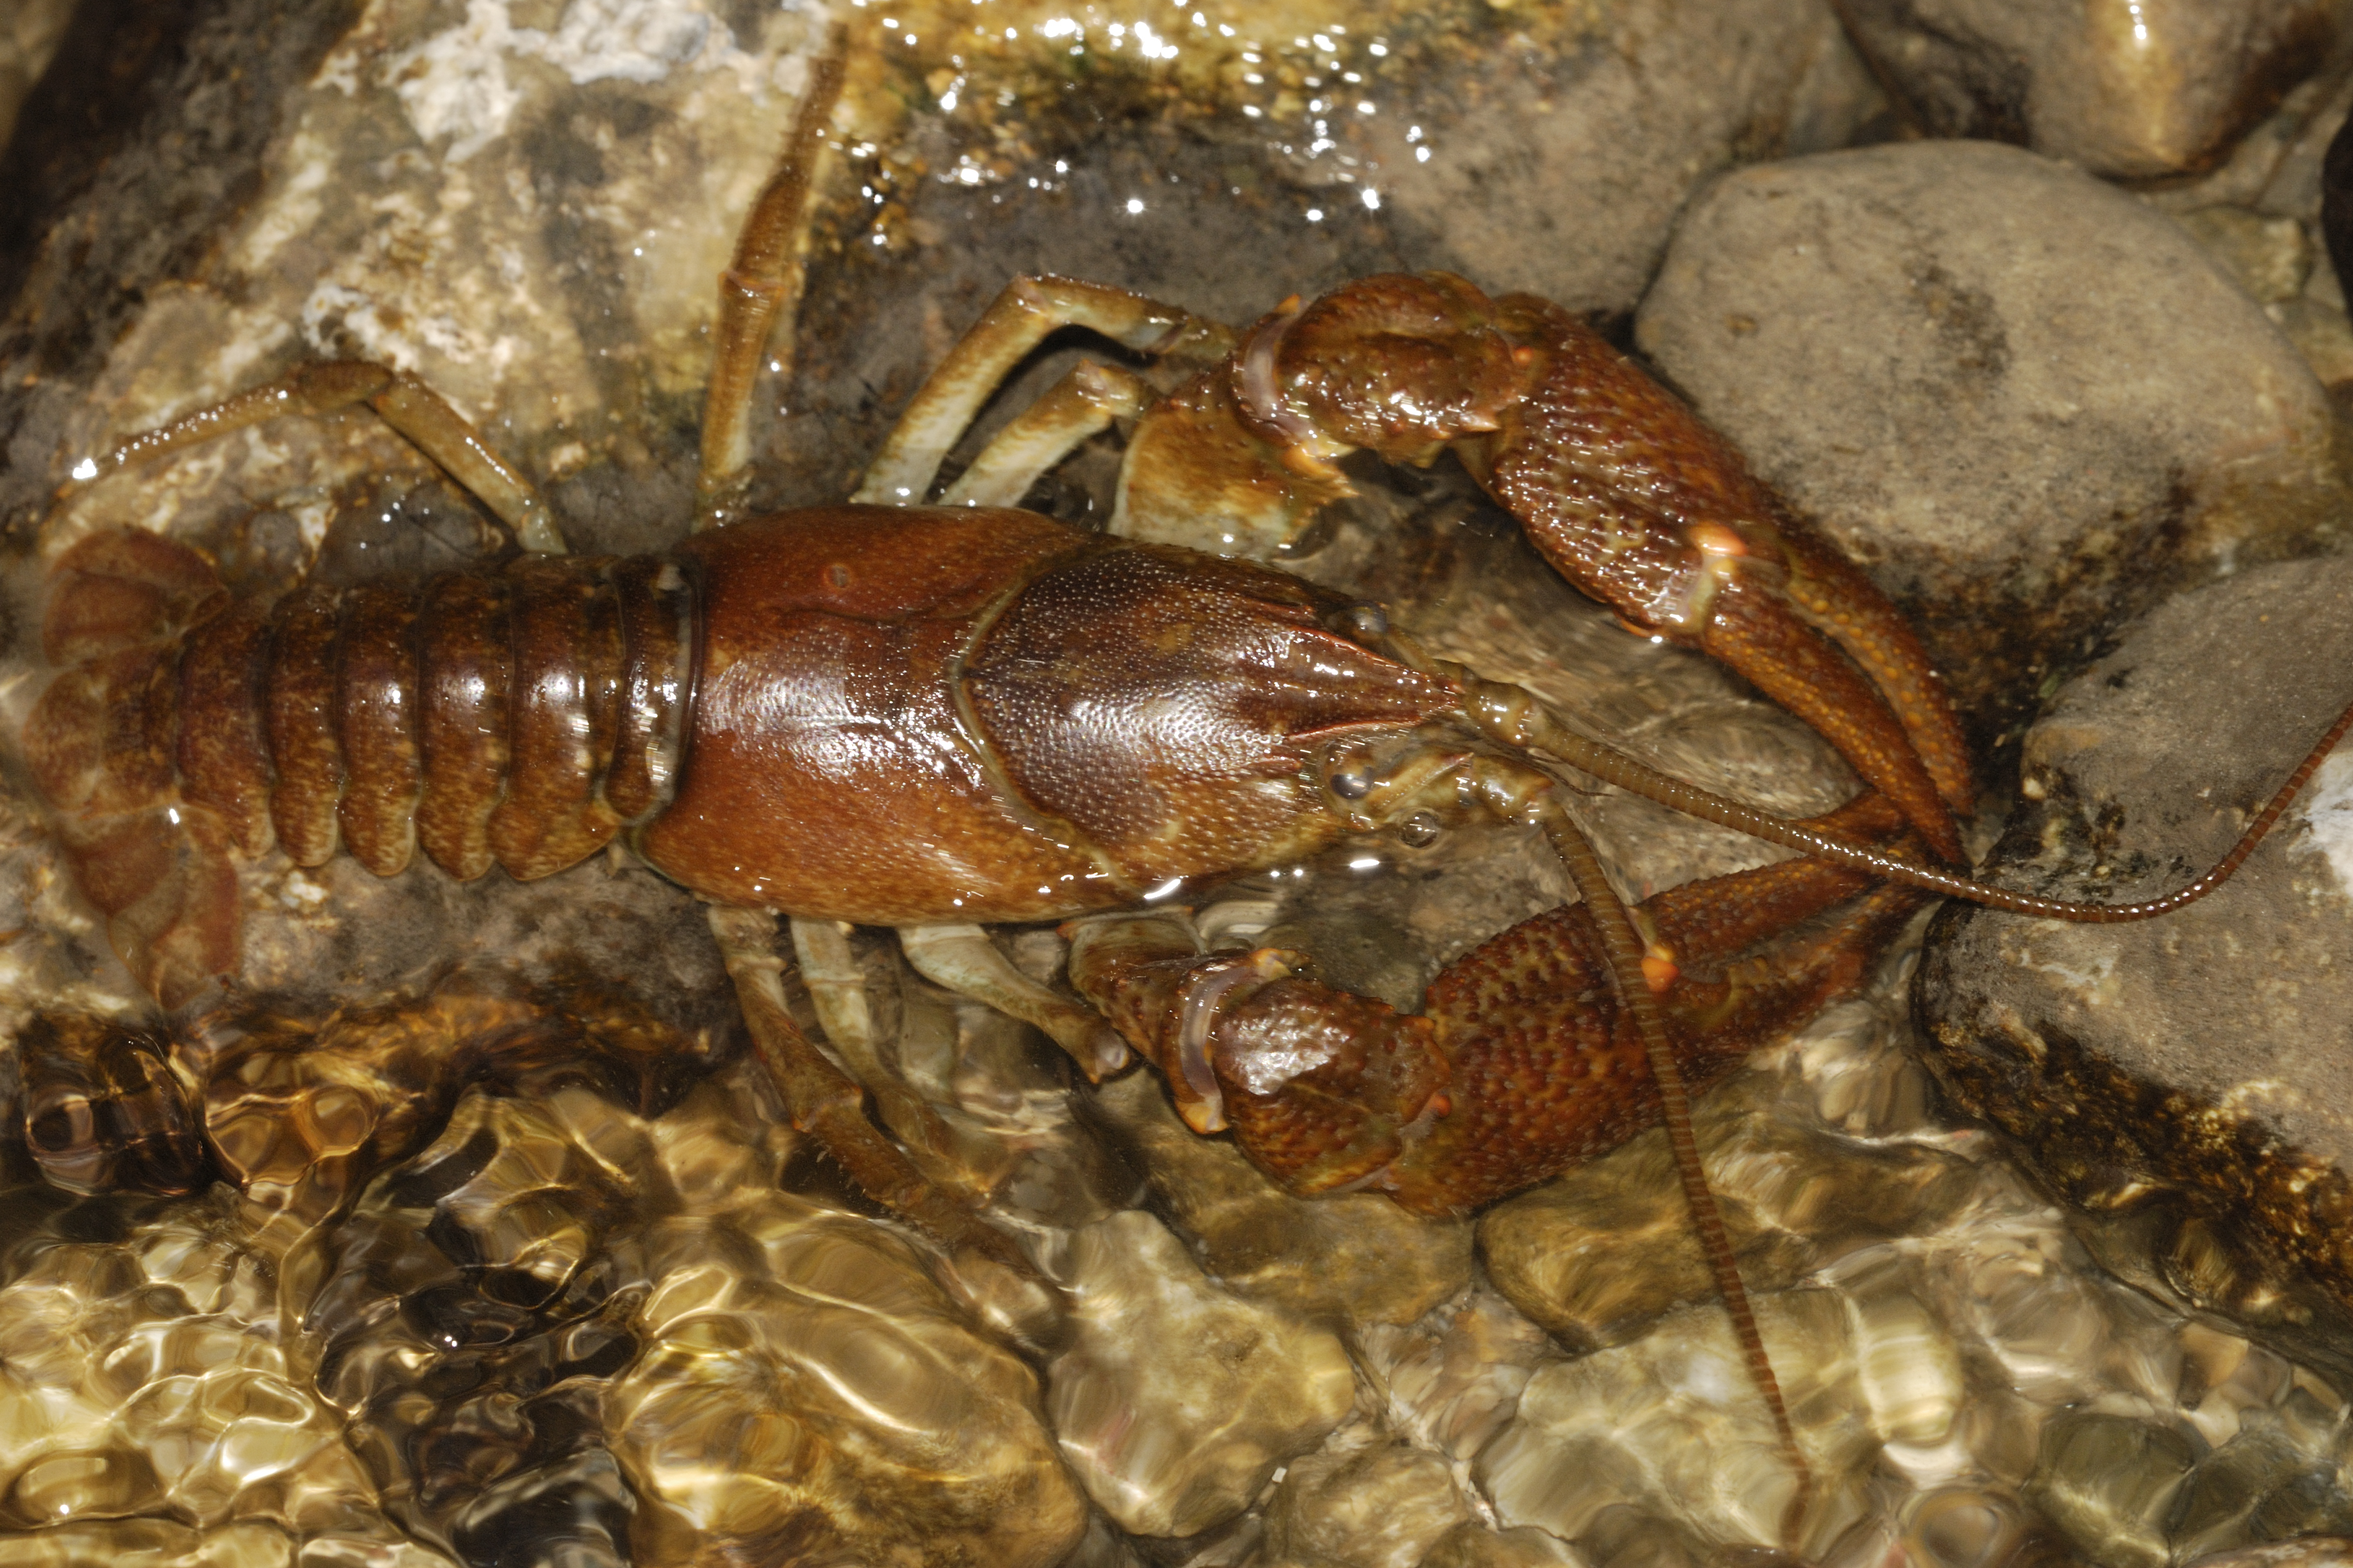
\includegraphics[width=\textwidth]{figs/Torrentium_ex1.jpg}
    \end{subfigure}
    \hfill
    \begin{subfigure}{0.45\textwidth}
        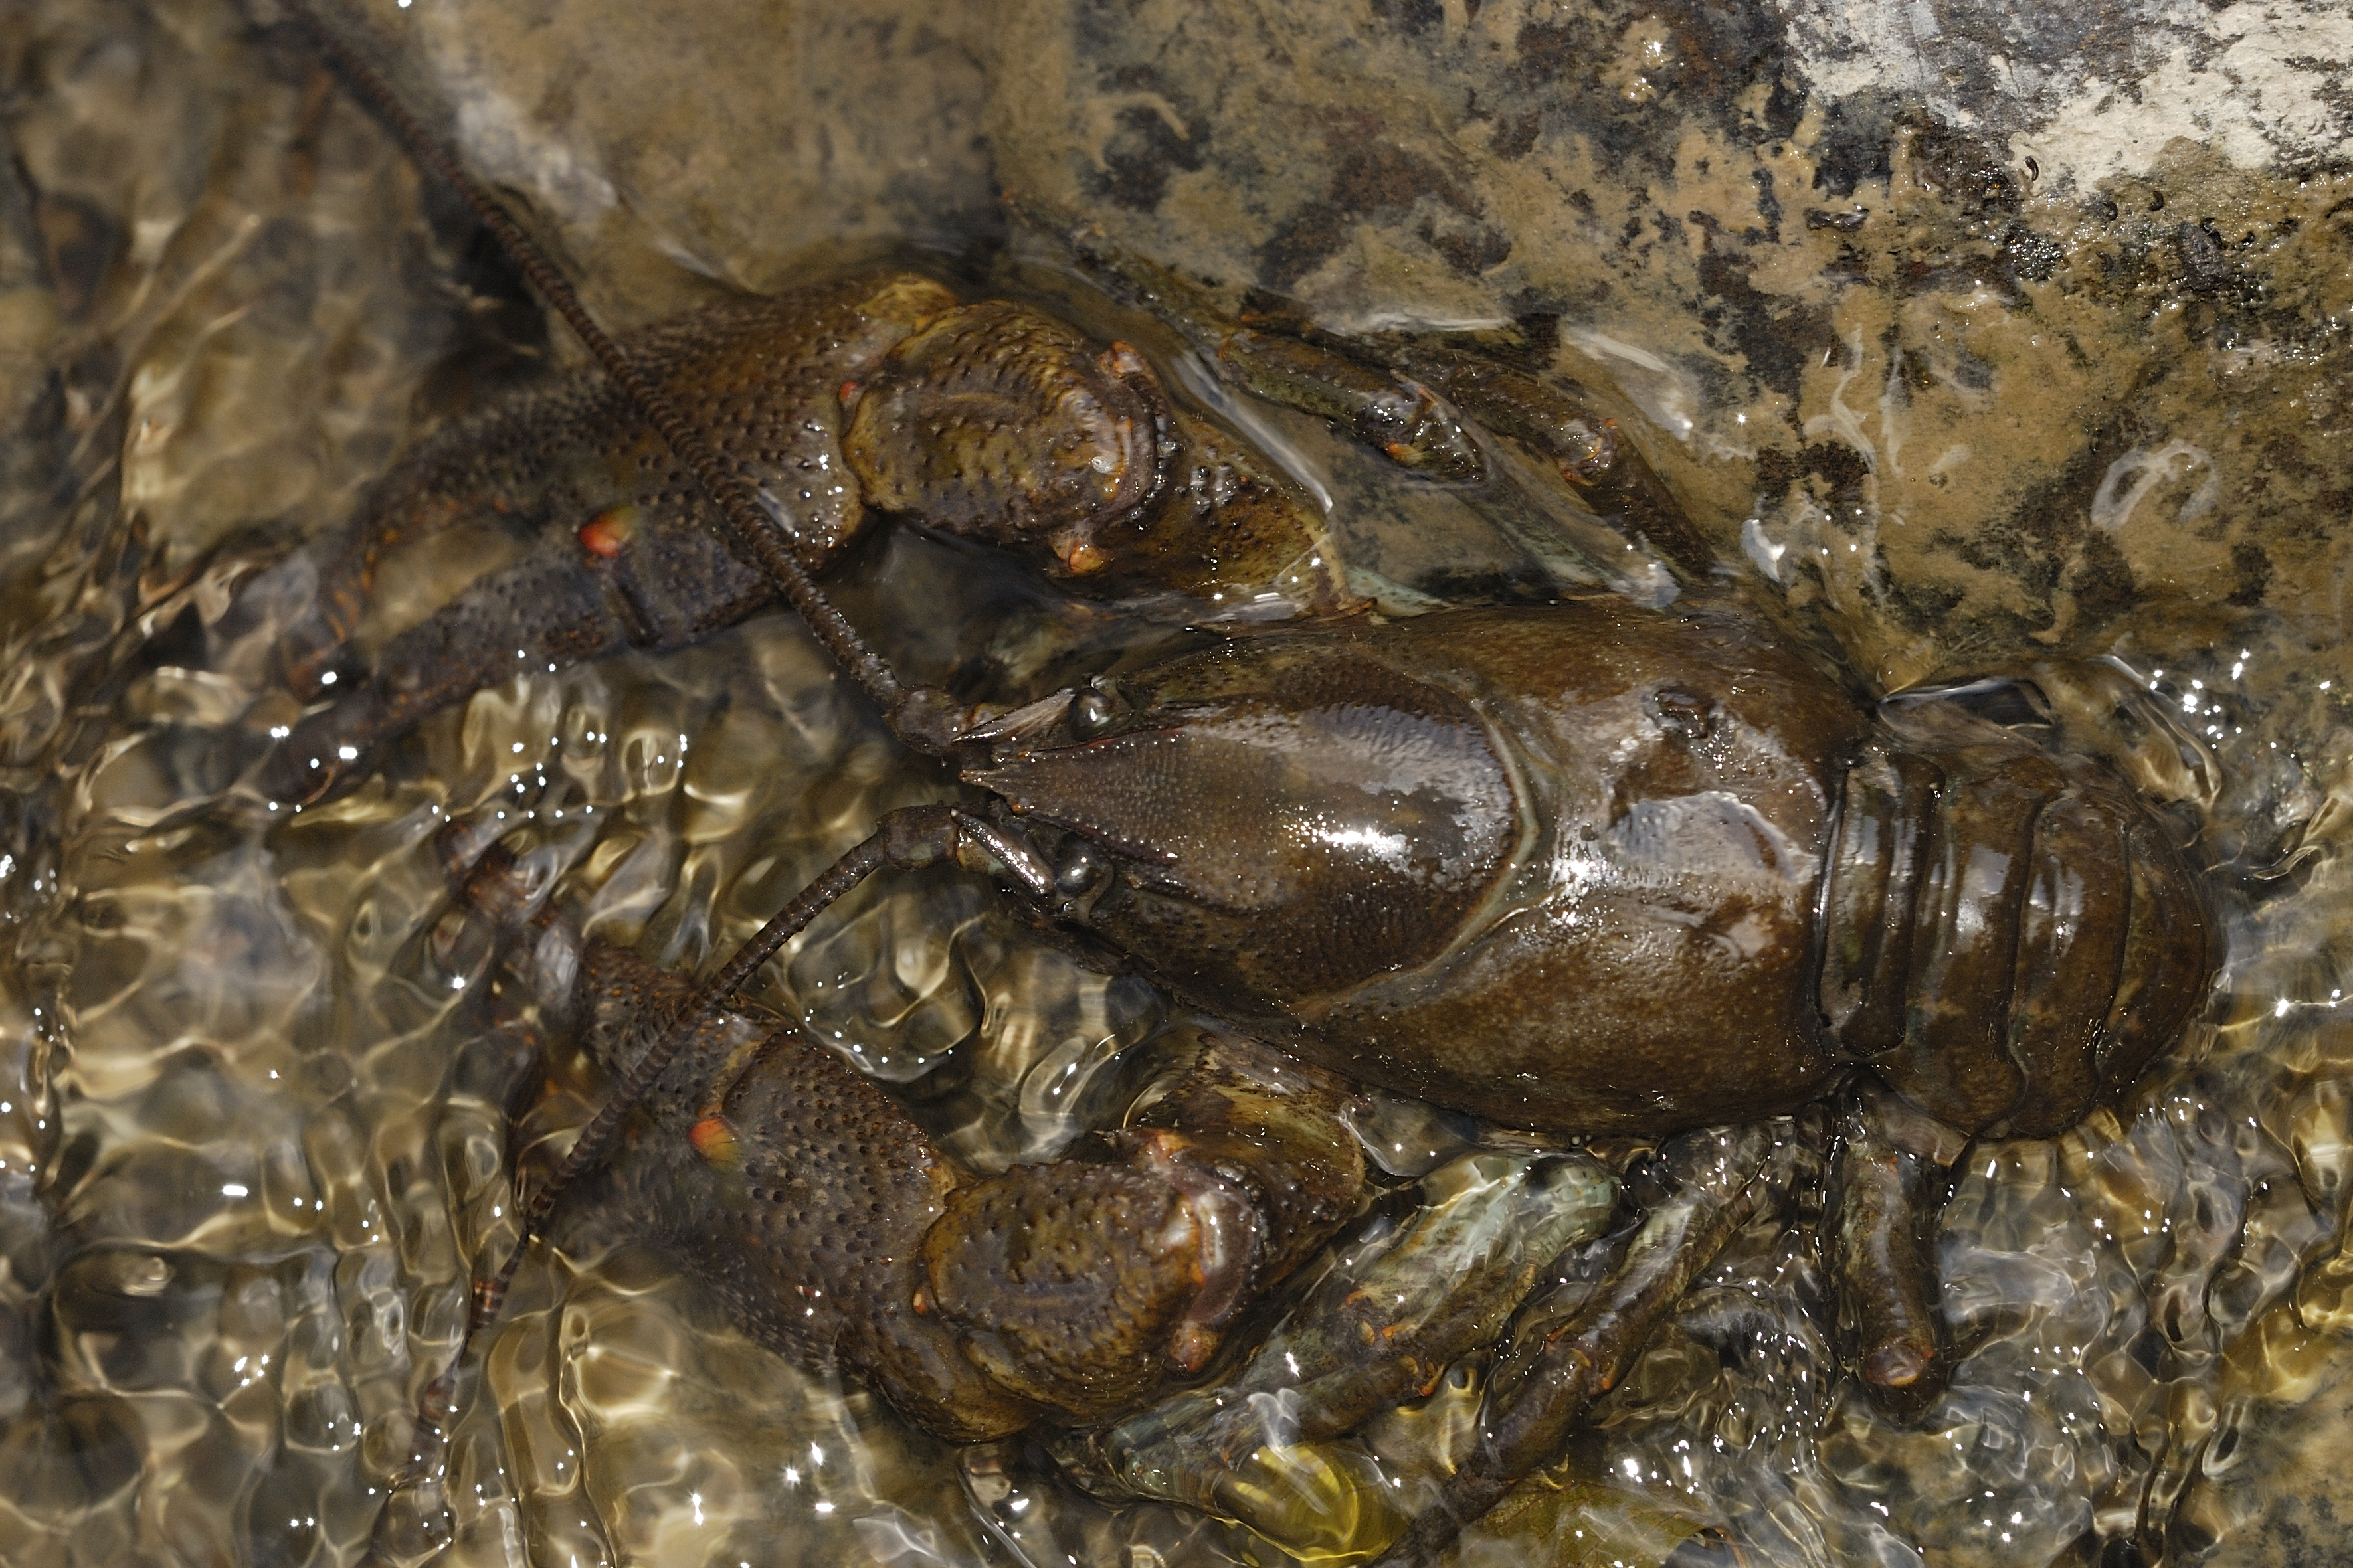
\includegraphics[width=\textwidth]{figs/Torrentium_ex2.jpg}
    \end{subfigure}
        \caption{Exemplare reprezentative de \textit{Austropotamobius
        bihariensis} (sus) și \textit{Austropotamobius torrentium} (jos),
        fotografiate în habitatul natural.}
    \label{fig:specii_raci}
\end{figure}



% exemple de imagini și caracteristici urmarite
% dificultati 
% exemple de imagini care pot conduce la concluzii
\section{Abordări existente}


Această secțiune prezintă lucrări recente în care sunt abordate probleme corelate cu cea studiată în această lucrare, axate pe identificarea automată a racilor prin tehnici de deep learning.


\subsection{Lightweight detection and segmentation of crayfish parts using an improved YOLOv11n model}

În lucrarea \cite{Lightweight_detection_and_segmentation_of_crayfish_parts_using_an_improved_YOLOv11n_segmentation_model}, autorii abordează problema detecției și segmentării sub-părților racilor (\textit{Procambarus clarkii}) în contexte industriale, unde este necesară o identificare precisă și rapidă a componentelor anatomice, precum cleștii, abdomenul, cefalotoracele și picioarele locomotoare. Problema este dificilă din cauza dimensiunilor reduse ale unor structuri, a ocluziilor frecvente și a scenelor aglomerate în care mai mulți indivizi se suprapun.

Metodologia propusă se bazează pe un model îmbunătățit de tip YOLOv11n-Seg (\textit{You Only Look Once version 11 nano -- Segmentation}), denumit YOLOv11n-DHBC. Autorii construiesc un set de date propriu, format inițial din 585 de imagini capturate la o rezoluție de 4032×3024 pixeli, utilizând un dispozitiv mobil, extins ulterior prin tehnici de augmentare la 3510 imagini. Setul de date este împărțit în subseturi de antrenare, validare și testare în raport 7:2:1, pentru a asigura o evaluare riguroasă a performanței modelului. Sunt definite patru clase de segmentare: cefalotorace, abdomen, clești și picioare locomotoare. Datele sunt etichetate manual la nivel de pixel folosind instrumentul LabelMe \cite{labelme} același instrument utilizat și în cadrul acestei lucrări pentru adnotarea imaginilor de rac.

Modelul introduce trei îmbunătățiri principale față de arhitectura de bază YOLOv11n-Seg: (1) un backbone D-HGNetV2 (\textit{Dynamic Hierarchical Graph Network version 2}), care integrează convoluții dinamice pentru o mai bună adaptare la variațiile datelor, reducând numărul de parametri cu 31\% față de modelul original; (2) un modul BiFPN (\textit{Bidirectional Feature Pyramid Network}) \cite{tan2020efficientdet}, utilizat pentru fuziunea bidirecțională a caracteristicilor multi-scală, cu ponderi învățabile care permit rețelei să determine autonom importanța fiecărei scări de reprezentare; și (3) un modul CARAFE (\textit{Content-Aware ReAssembly of FEatures}) \cite{wang2019carafe}, utilizat pentru upsampling adaptiv în locul interpolării nearest-neighbor clasice, care păstrează detaliile fine ale obiectelor mici.

Rezultatele experimentale arată că modelul propus atinge o performanță ridicată, obținând un mAP@0.5 de 96.8\% pentru detecție prin bounding box și 96.0\% pentru segmentare la nivel de instanță, depășind astfel performanțele modelului de bază YOLOv11n-Seg. Modelul este eficient din punct de vedere computațional, având doar 2.0 milioane de parametri și o dimensiune de 4.2 MB, putând rula în timp real la 65.8 cadre pe secundă (FPS).

Avantajele metodei includ un echilibru bun între acuratețe și eficiență, capacitatea de a gestiona obiecte mici și ocluzionate, precum și posibilitatea de implementare pe dispozitive cu resurse limitate (\textit{edge devices}). Limitările constau în dificultăți persistente în segmentarea completă a structurilor anatomice foarte mici în scenarii extrem de aglomerate și în dependența de un set de date specific domeniului industrial.

Comparativ cu alte metode evaluate, precum Mask R-CNN, YOLOv5s, YOLOv7 și YOLOv8n, modelul propus oferă o performanță similară sau superioară în termeni de acuratețe, cu un cost computațional considerabil mai redus, acesta fiind mai adecvat pentru aplicații industriale în timp real.

Față de abordarea prezentată în această lucrare, metoda propusă de Shi et al. \cite{Lightweight_detection_and_segmentation_of_crayfish_parts_using_an_improved_YOLOv11n_segmentation_model} se diferențiază atât prin natura problemei, cât și prin mijloacele tehnice utilizate. În timp ce lucrarea citată urmărește segmentarea sub-părților unui singur individ dintr-o singură specie (\textit{P. clarkii}), în contexte industriale cu imagini dense, această lucrare abordează clasificarea interspecifică binară la nivelul specimenului întreg, pe imaginile recoltate direct din habitatul natural. Arhitectura AlexNet cu transfer learning de la ImageNet, utilizată în această lucrare, este mult mai simplă și mai potrivită pentru un set de date de dimensiuni reduse (sub 320 de imagini originale), comparativ cu modelul YOLO de ultimă generație antrenat pe mii de imagini augmentate.




\subsection{Research on the Identification Algorithm of Crayfish Body Features Based on the Improved YOLOv8n Loss Function}

În lucrarea \cite{Identification_Algorithm_of_Crayfish_Body_Features_Based_on_the_Improved_YOLOv8n_Loss_Function}, autorii abordează detecția și identificarea diferitelor părți anatomice ale racilor (\textit{Procambarus clarkii}), cu scopul de a îmbunătăți procesele automate din acvacultură, precum sortarea și monitorizarea calității specimenelor. Dificultățile principale sunt generate de suprapunerea bounding box-urilor datorită volumului mare al chelelor, variațiile de poziție ale racilor și diferențele de formă ale componentelor anatomice.

Abordarea propusă se bazează pe modelul YOLOv8n (\textit{You Only Look Once version 8 nano}), ales pentru eficiența sa computațională. Setul de date conține 1073 de imagini capturate în mediu de laborator, pe fundal alb, pentru a asigura consistența datelor și o mai bună generalizare. Datorită dimensiunii reduse a setului de date, autorii aplică tehnici de augmentare: oglindire (\textit{flip}), conversie în tonuri de gri și adăugare de zgomot. Datele sunt etichetate folosind LabelImg \cite{labelimg}, cu trei clase principale: corp (\textit{Crayfish}), clești și picioare locomotoare (\textit{Aofoot}) și coadă (\textit{Tail}). Setul de date este împărțit în subseturi de antrenare și validare în raport 9:1.

Contribuția principală a lucrării constă în înlocuirea funcției de pierdere  utilizate în regresia bounding box-urilor. Funcția CIoU (\textit{Complete Intersection over Union}), utilizată implicit în YOLOv8, este înlocuită cu o combinație între Inner IoU și MPDIoU (\textit{Minimum Point Distance Intersection over Union}). Inner IoU utilizează bounding box-uri auxiliare scalate printr-un factor de proporție pentru a îmbunătăți procesul de învățare în cazul suprapunerilor, iar MPDIoU optimizează distanța euclidiană dintre colțurile bounding box-urilor pentru o localizare mai precisă atunci când raportul de aspect al predicției coincide cu cel al adevărului fundamental.

Modelul îmbunătățit obține performanțe ridicate: precizie de 99.3\%, recall de 99.7\% și un mAP@0.5:0.95 de 90.8\%. Studiile de ablație arată că introducerea Inner IoU și MPDIoU conduce la o creștere a mAP@0.5:0.95 cu 7.1 puncte procentuale față de modelul YOLOv8n original (83.7\%). La nivelul claselor individuale, cel mai dificil de detectat rămâne coada, cu un mAP de doar 83.5\%, datorită tendinței acesteia de a fi curbată și acoperită de corp în imagini.

Avantajele metodei includ acuratețea ridicată și o mai bună gestionare a suprapunerilor dintre bounding box-uri, precum și o convergență mai rapidă a modelului față de YOLOv5s și SSD. Limitările constau în utilizarea unui set de date relativ redus captat exclusiv pe fundal alb de laborator, ceea ce poate afecta generalizarea în scenarii reale cu fundal natural complex. Detectarea cozii rămâne dificilă în situațiile în care aceasta este ocluzionată sau curbată pe corp.

Comparativ cu SSD și YOLOv5s evaluate în aceeași lucrare, modelul propus oferă un echilibru mai bun între acuratețe și eficiență computațională: SSD a obținut o acuratețe medie de doar 76\%, cu o performanță deosebit de slabă la identificarea cozii (47\%). Spre deosebire de abordările bazate pe segmentare la nivel de pixel, această metodă utilizează doar detecție pe bază de bounding box-uri, ceea ce reduce costul computațional, dar limitează precizia delimitării exacte a obiectelor.

Față de abordarea din această lucrare, metoda propusă de Islam et al. \cite{Identification_Algorithm_of_Crayfish_Body_Features_Based_on_the_Improved_YOLOv8n_Loss_Function} se diferențiază pe mai multe planuri. În primul rând, problema vizată este diferită: lucrarea citată urmărește detectarea sub-părților anatomice ale unui individ din cadrul aceleiași specii comerciale, în timp ce această lucrare rezolvă o problemă de clasificare interspecifică între două specii protejate cu morfologie similară, \textit{A. bihariensis} și \textit{A. torrentium}. În al doilea rând, imaginile utilizate în lucrarea citată sunt capturate în condiții controlate de laborator, pe fundal alb și uniform, ceea ce simplifică semnificativ sarcina de detecție; în schimb, setul de date utilizat în această lucrare provine din teren, cu fundaluri naturale variate și condiții de iluminare necontrolate. În al treilea rând, arhitectura AlexNet cu straturi convoluționale înghețate și transfer learning de la ImageNet este adecvată pentru clasificare binară pe un set de date mic, fără a necesita modificări ale funcției de pierdere sau tehnici specializate de regresie a bounding box-urilor.



\subsection{Application of Improved YOLOv8n-seg in Crayfish Trunk Segmentation}

În lucrarea \cite{Application_of_Improved_YOLOv8n-seg_in_Crayfish_Trunk_Segmentation}, autorii abordează problema segmentării trunchiului principal al racilor (\textit{Procambarus clarkii}) în vederea gradării automate a specimenelor comerciale în funcție de specificații. Scopul aplicației este practic: după segmentare, aria în pixeli a trunchiului este convertită în greutate corporală reală, eliminând necesitatea inspecției vizuale manuale în liniile de procesare industrială.


Metodologia propusă introduce algoritmul GHBSeg-YOLOv8, construit pe baza modelului YOLOv8n-seg, cu trei îmbunătățiri structurale principale. Prima constă în înlocuirea rețelei backbone originale cu o arhitectură hibridă GhostHGNetV2, care combină modulul GhostNet \cite{han2020ghostnet} (ce generează hărți de caracteristici suplimentare prin transformări liniare simple aplicate unui număr redus de convoluții de bază, reducând astfel complexitatea computațională) cu rețeaua HGNetV2 \cite{pphgnetv2}, dezvoltată în cadrul framework-ului PaddlePaddle al companiei Baidu, bazată pe extragerea ierarhică a caracteristicilor la scări multiple. A doua îmbunătățire constă în introducerea modulului BiFPN (\textit{Bidirectional Feature Pyramid Network}) \cite{tan2020efficientdet} în rețeaua neck, pentru fuziunea multi-scală bidirecțională cu ponderi adaptive care permit modelului să ajusteze importanța fiecărei scări de reprezentare. A treia îmbunătățire constă în utilizarea convoluțiilor separabile în adâncime pentru transformarea liniară a trăsăturilor, contribuind suplimentar la reducerea numărului de parametri.


Setul de date a fost construit de autori, conținând 234 de imagini achiziționate cu un sistem de cameră industrială (HIKVISION MV-CS050-10GC, rezoluție 2248×2048 pixeli) pe fundal alb uniform, completate cu imagini suplimentare capturate cu telefonul mobil din unghiuri și înălțimi diferite pentru a crește diversitatea datelor. Prin tehnici de augmentare (oglindire, conversie în tonuri de gri și adăugare de zgomot), setul a fost extins la 1038 de imagini. Adnotarea a utilizat instrumentul LabelMe la nivel de contur al trunchiului, cu împărțire antrenare/validare în raport 9:1 și 200 de epoci de antrenare.

Rezultatele din experimentele comparative demonstrează că modelul GHBSeg-YOLOv8 reduce numărul de parametri cu 60.5\% față de YOLOv8n-seg original (de la 3.25M la 1.28M) și dimensiunea modelului cu 55.4\% (de la 6.5MB la 2.9MB), îmbunătățind totodată mAP de la 98.9\% la 99.2\%. Numărul de operații în virgulă mobilă scade de la 12.0 GFLOPs la 5.8 GFLOPs. Comparativ cu modele alternative evaluate, inclusiv Mask R-CNN (mAP 88.9\%, 43.9M parametri, 244MB), DeepLabV3+ (mAP 78.6\%) și YOLOv5-seg (mAP 96.4\%), GHBSeg-YOLOv8 obține cel mai bun echilibru între acuratețe și eficiență computațională dintre toate modelele testate.

Avantajele metodei constau în dimensiunea redusă a modelului final (2.9MB), compatibilă cu implementarea pe dispozitive mobile și plăci de dezvoltare embedded, și în acuratețea ridicată a segmentării pe o singură clasă morfologică. Limitările declarate de autori vizează faptul că experimentele au fost conduse exclusiv în mediu de laborator controlat (fundal alb și uniform), ceea ce poate limita generalizarea la scenarii reale cu fundal natural și posturi dinamice ale racilor.

Față de abordarea din această lucrare, metoda propusă de Geng et al. \cite{Application_of_Improved_YOLOv8n-seg_in_Crayfish_Trunk_Segmentation} se diferențiază în mai multe privințe. În primul rând, obiectivul este distinct: lucrarea citată urmărește segmentarea la nivel de pixel a trunchiului unui singur individ dintr-o singură specie comercială în scopul gradării industriale, în timp ce această lucrare rezolvă clasificarea interspecifică binară a două specii protejate cu morfologie similară, \textit{A. bihariensis} și \textit{A. torrentium}. În al doilea rând, datele utilizate de Geng et al. provin exclusiv din mediu de laborator cu fundal alb și echipamente industriale de achiziție, simplificând considerabil sarcina de segmentare; setul de date utilizat în această lucrare provine din teren, cu fundal natural variat și condiții de iluminare necontrolate. În al treilea rând, arhitectura AlexNet cu straturi convoluționale înghețate și transfer learning de la ImageNet este adecvată pentru clasificare binară pe un set de date mic, fără a necesita segmentare la nivel de pixel, modificări ale arhitecturii backbone sau estimarea greutății corporale.

Tabelul~\ref{tab:comparatie_yolo} sumarizează principalele caracteristici, rezultate experimentale și limitări ale celor trei lucrări prezentate, evidențiind diferențele de set de date, metodologie și performanță față de abordarea propusă în această lucrare.

\begin{table}[H]
\centering
\caption{Comparație între lucrările bazate pe YOLO discutate în
această secțiune și abordarea propusă în această lucrare.}
\label{tab:comparatie_yolo}
\begin{tabular}{p{1.6cm}p{1.9cm}p{2.2cm}p{2.4cm}p{2.7cm}}
\hline
\textbf{Lucrare} & \textbf{Model} & \textbf{Set de date} &
\textbf{Rezultate principale} & \textbf{Limitări principale} \\
\hline
Shi et al. \cite{Lightweight_detection_and_segmentation_of_crayfish_parts_using_an_improved_YOLOv11n_segmentation_model} &
YOLOv11n-DHBC &
585$\rightarrow$3510 imagini augmentate, \textit{P. clarkii} &
mAP@0.5: 96.8\% (detecție), 96.0\% (segmentare); 65.8 FPS &
Dificultăți la structuri mici în scene aglomerate; set specific industrial \\
\hline
Islam et al. \cite{Identification_Algorithm_of_Crayfish_Body_Features_Based_on_the_Improved_YOLOv8n_Loss_Function} &
YOLOv8n + Inner IoU/MPDIoU &
1073 imagini, fundal alb laborator, \textit{P. clarkii} &
Precizie 99.3\%; Recall 99.7\%; mAP@0.5:0.95 90.8\% &
Set redus, doar fundal alb; detectarea cozii rămâne dificilă (mAP 83.5\%) \\
\hline
Geng et al. \cite{Application_of_Improved_YOLOv8n-seg_in_Crayfish_Trunk_Segmentation} &
GHBSeg-YOLOv8 &
234$\rightarrow$1038 imagini augmentate, fundal alb, \textit{P. clarkii} &
mAP 99.2\%; 1.28M parametri; 2.9MB &
Doar mediu de laborator controlat; o singură clasă morfologică \\
\hline
\textbf{Această lucrare} &
\textbf{AlexNet + transfer learning} &
318 imagini originale, teren natural, \textit{A. bihariensis}/\textit{A. torrentium} &
Acuratețe test 95.92\% &
Set redus; adnotare manuală prealabilă necesară \\
\hline
\end{tabular}
\end{table}


\subsection{Sumar}

Lucrările prezentate în această secțiune abordează probleme conexe identificării speciilor de raci, dar diferă fundamental de demersul propus aici prin natura sarcinii, speciile vizate și condițiile de colectare a datelor. Shi et al. \cite{Lightweight_detection_and_segmentation_of_crayfish_parts_using_an_improved_YOLOv11n_segmentation_model}, Islam et al. \cite{Identification_Algorithm_of_Crayfish_Body_Features_Based_on_the_Improved_YOLOv8n_Loss_Function} și Geng et al. \cite{Application_of_Improved_YOLOv8n-seg_in_Crayfish_Trunk_Segmentation} rezolvă sarcini de detecție și segmentare a sub-părților anatomice ale unui singur individ, dintr-o singură specie comercială (\textit{Procambarus clarkii}), pe seturi de date de dimensiuni medii spre mari (1073--3510 imagini, după augmentare), capturate fie în mediu de laborator controlat, fie cu echipamente industriale specializate.

Această lucrare abordează, în schimb, o problemă de clasificare interspecifică binară: distingerea între două specii protejate cu morfologie similară, \textit{A. bihariensis} și \textit{A. torrentium}, pe baza unor imagini de teren colectate în habitatul natural, cu fundal variabil și condiții de iluminare necontrolate. Dimensiunea setului de date propriu (318 imagini) este considerabil mai redusă decât în lucrările citate, reflectând dificultatea practică a colectării de date pentru specii protejate, cu populații limitate și acces restricționat în teren.

Din punct de vedere metodologic, cele trei lucrări citate utilizează arhitecturi YOLO moderne, optimizate pentru detecție și segmentare în timp real, cu module suplimentare (BiFPN, CARAFE, GhostHGNetV2) care vizează echilibrul dintre acuratețe și eficiență computațională. În contrast, această lucrare adoptă arhitectura AlexNet \cite{krizhevsky2012imagenet}, mai simplă din punct de vedere structural, dar adaptată prin transfer learning de la ImageNet: ponderile straturilor convoluționale sunt menținute înghețate, iar stratul de ieșire este înlocuit pentru clasificarea binară a celor două specii. Această abordare valorifică reprezentările vizuale generale învățate pe un set de date masiv, compensând astfel dimensiunea redusă a setului de date propriu, pentru care antrenarea de la zero a unei arhitecturi moderne ar conduce inevitabil la supra-antrenare.

Diferența fundamentală de task (clasificare la nivel de imagine, față de detecție sau segmentare la nivel de sub-parte sau individ), de specii vizate (specii protejate cu acces limitat, față de o specie comercială larg disponibilă) și de condiții de colectare a datelor (teren necontrolat, față de mediu de laborator sau industrial) face imposibilă o comparație numerică directă a performanțelor raportate. Cu toate acestea, abordarea propusă demonstrează că transfer learning-ul reprezintă o soluție viabilă și pentru seturi de date considerabil mai mici decât cele utilizate în lucrările citate, situație frecventă în studiile de biodiversitate pe specii protejate.




% prezentare lucrari care au abordat aceeași problema sau probleme similare
% pt fiecare lucrare:
%  1. problema abordata 
%  2. metodele folosite:  set de date, preprocesari, modele
%  3. rezultate obtinute
%  4. avantaje si dezavantaje/eventuale limitari 
%  5. cum se diferentiaza metoda utilizata de tine de metoda descris